%! Author = gacou54

% Preamble
\documentclass[11pt]{article}

% Packages
\usepackage{amsmath}
\usepackage{hyperref}
\usepackage{listings}

\usepackage{tikz}
\usetikzlibrary{arrows}
\usetikzlibrary{shapes}
\usepackage{xcolor}


% Document information
\title{Othello User Guide}
\author{Gabriel Couture}
\setcounter{tocdepth}{2}

% Document
\begin{document}

    \maketitle
    \tableofcontents
    \newpage


    \section{Introduction}\label{sec:introduction}
    Othello is a tool that allows you to link optimization data from Macbeth software
    and geographic data in GDB format (ArcGIS proprietary format).
    It consists of two tools: the first being \textit{Criteria}, and the second \textit{Aggregate}.

    \subsection{\textit{Criteria}}\label{subsec:criteria}
    The \textit{Criteria} allows to transform the values of a criterion thanks
    to a scale present in a macbeth file. 

    \begin{figure}[h]
        \centering
        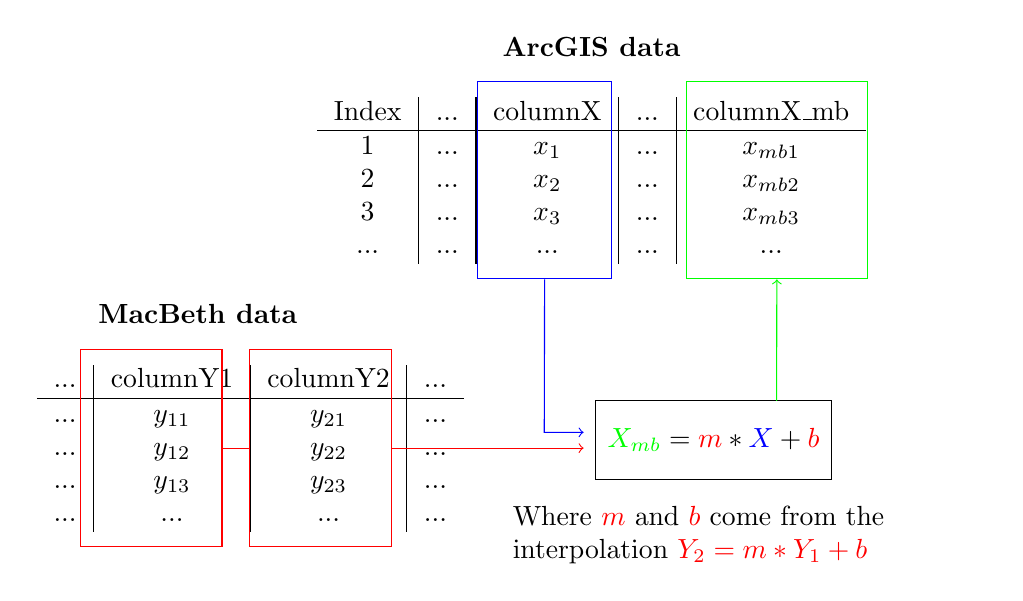
\begin{tikzpicture}
    % Tables
    \node (tab1) {%
        \begin{tabular}{c|c|c|c|c}
            Index  & ... & columnX & ... & columnX\_mb \\
            \hline
            1 & ... & $x_1$ & ... & $x_{mb1}$ \\
            2 & ... & $x_2$ & ... & $x_{mb2}$ \\
            3 & ... & $x_3$ & ... & $x_{mb3}$ \\
            ... & ... & ... & ... & ...
        \end{tabular}
    };
    \node [left,xshift=-1.5cm,yshift=-3.4cm] (tab2) {%
        \begin{tabular}{c|c|c|c}
            ... & columnY1 & columnY2 & ...\\
            \hline
            ... & $y_{11}$ & $y_{21}$ & ...\\
            ... & $y_{12}$ & $y_{22}$ & ...\\
            ... & $y_{13}$ & $y_{23}$ & ... \\
            ... & ... & ... & ...
        \end{tabular}
    };

    % Table labels
    \node[yshift=1.7cm] {\textbf{ArcGIS data}};
    \node[xshift=-5cm, yshift=-1.7cm] {\textbf{MacBeth data}};

    % Rectangles
    \node [
        rectangle,
        draw=blue,
        right,
        xshift=-1.45cm,
        minimum width=1.7cm,
        minimum height=2.5cm,
    ] (rec-x) {};
    \node [
        rectangle,
        draw=red,
        right,
        xshift=-6.5cm,
        yshift=-3.4cm,
        minimum width=1.8cm,
        minimum height=2.5cm,
    ] (rec-y1) {};
    \node [
        rectangle,
        draw=red,
        right,
        xshift=-4.35cm,
        yshift=-3.4cm,
        minimum width=1.8cm,
        minimum height=2.5cm,
    ] (rec-y2) {};
    \node [
        rectangle,
        draw=green,
        right,
        xshift=1.2cm,
        minimum width=2.3cm,
        minimum height=2.5cm,
    ] (rec-mb) {};
    \node [
        draw,
        rectangle,
        xshift=1.55cm,
        yshift=-3.3cm,
        minimum width=3cm,
        minimum height=1cm,
    ] (rec) {
        $\textcolor{green}{X_{mb}} = \textcolor{red}{m} * \textcolor{blue}{X} + \textcolor{red}{b}$
    };

    % Labels
    \node [xshift=2cm, yshift=-4.5cm, text width=6cm] {
        Where $\textcolor{red}{m}$ and $\textcolor{red}{b}$ come from the\\
        interpolation $\color{red} Y_2 = m * Y_1 + b$
    };

    % Arrows
    \draw [->, blue] (rec-x) -- (-0.6cm,-3.2cm) -- (-0.1cm,-3.2cm);
    \draw [-, red] (rec-y1) -- (rec-y2);
    \draw [->, red] (rec-y2) -- (-0.1cm,-3.4cm);
    \draw [->, green] (2.35cm,-2.8cm) -- (rec-mb);

\end{tikzpicture}
        \caption{Criteria tool data flow diagram}
        \label{fig:criteria-tool}
    \end{figure}

    \subsection{\textit{Aggregate}}\label{subsec:aggregate}


    \section{Installation}\label{sec:installation}

    \subsection{Install from release (preferred)}\label{subsec:install-from-release-(preferred)}
    \begin{enumerate}
        \item Find the most recent release here: \url{https://github.com/ulaval-rs/othello/releases}
        \item In the assets, download the othello zip file
        \item Unzip the zip file at the path where you want the application
        \item Run \texttt{app.exe} to start the application
    \end{enumerate}

    \subsection{Install from source}\label{subsec:install-from-source}
    Clone the repo


    \section{Usage}\label{sec:usage}
    TODO

\end{document}
